%
% Chapter 2 - Requirements and project's structure
%

\chapter{Requirements and project's structure}

\section{Requirements analysis}

In order to build this multiplaform application a relational database and a HTTP server must be included
in the backend, which will store and supply information to the two clients: the mobile application and the web browser application.

\subsection{Database}

\subsubsection{Functional requirements}

\begin{itemize}
    \item Store user information and submissions;
    \item Seperate data, labeling which ones should be votable, favorable or reportable;
\end{itemize}

\subsubsection{Non-functional requirements}

\begin{itemize}
    \item Support encrypted tuples;
\end{itemize}

\subsection{HTTP Server}

\subsubsection{Functional requirements}

\begin{itemize}
    \item Provide lists from restaurants and their meals;
    \item Allow the clients to add restaurants and meals;
    \item Provide the ability to vote on other user's content to filter the information and provide self-maintainability;
    \item Provide the ability to report in case of corrupt / voided submits;
    \item Provide restaurants and meals information based on the user geolocation;
\end{itemize}

\subsubsection{Non-functional requirements}

\begin{itemize}
    \item Provide user credentials encryption when registering;
    \item Encrypt user sensitive information when inserting them into the database, like insulin profiles;
\end{itemize}

\subsection{Mobile application}

\subsubsection{Functional requirements}

\begin{itemize}
    \item Show lists and detailed information that is provided by the HTTP server;
    \item Allow the user to create insulin profiles;
    \item Insulin dosage calculation based on the current user's blood glucose;
    \item Allow the user to vote, report and add content to its personal favorites;
    \item Give the ability to login and logout from the user account;
\end{itemize}

\subsubsection{Non-functional requirements}

\begin{itemize}
    \item Allow the user to choose its default measurement units;
    \item Allow user registering;
\end{itemize}

\subsection{Front web application}

\subsubsection{Functional requirements}

\begin{itemize}
    \item Platform administration tools;
    \item Faulty data management;
    \item User control;
\end{itemize}

\subsubsection{Non-functional requirements}

\begin{itemize}
    \item TODO
\end{itemize}

\section{Project's structure}

To match the previously stated requirements the group managed to conceive a platform following the structure
represented by the next picture:\\

\begin{figure}[H]
    \begin{center}
        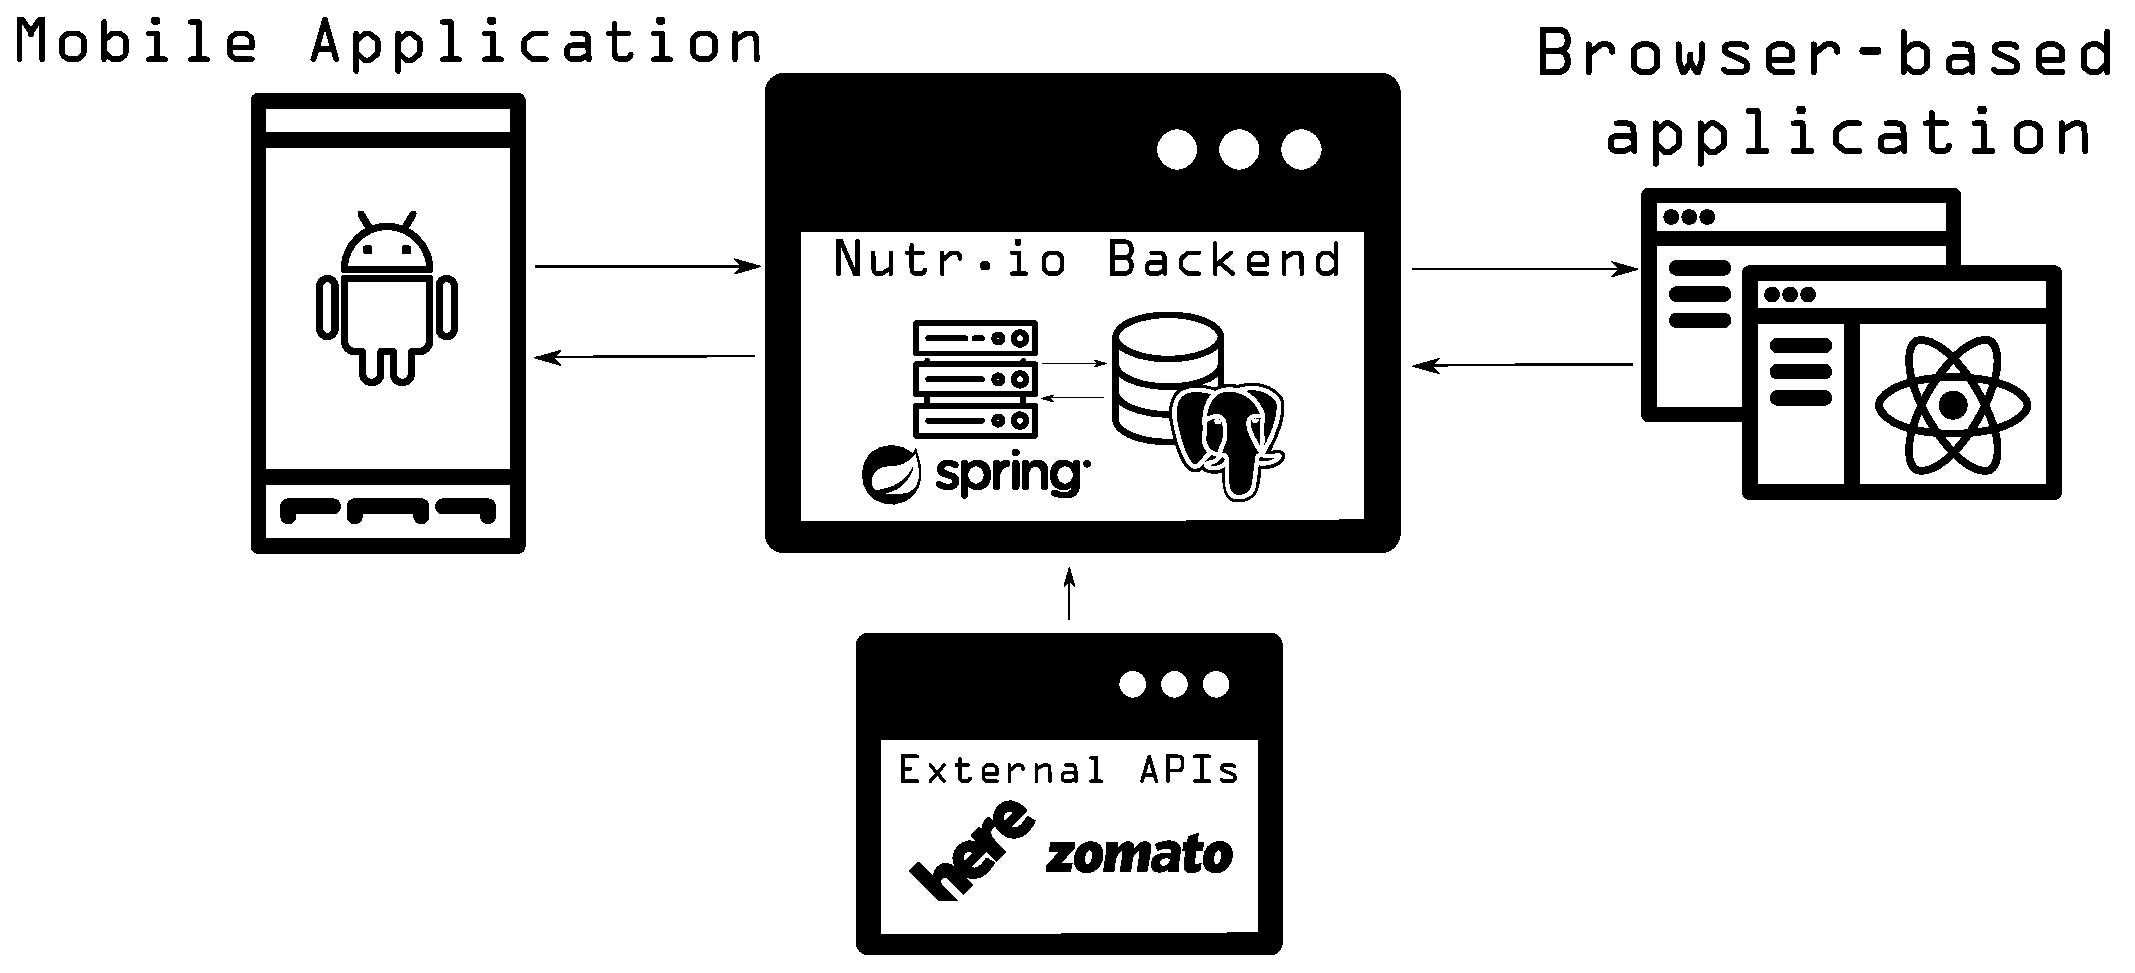
\includegraphics[scale=0.4]{_figures/Nutrio_components.eps}
        \caption{Nutr.io platform components}
    \end{center}
\end{figure}

As shown, the platform will be composed by two clients: a mobile application for Android devices and a web browser
application, which will have as backend a HTTP server and a relational database.\\

External APIs will also be used to obtain restaurants' related information. After some discussion, the group chose
to use the Here API, to provide restaurant information and geolocation.\\

More details about the chosen tecnologies for each component will be described in the fourth chapter of this report.\\